%%%%%%%%%%%%%%%%%%%%%%%%%%%%%%%%%%%%%%%%%%%%%%%%%%%%%%%%
%                IAML 2020 Assignment 2                %
%                                                      %
%                                                      %
% Authors: Hiroshi Shimodaira and JinHong Lu           %
% Based on: Assignment 1 by Oisin Mac Aodha, and       %
%          Octave Mariotti                             %
% Using template from: Michael P. J. Camilleri and     %
% Traiko Dinev.                                        %
%                                                      %
% Based on the Cleese Assignment Template for Students %
% from http://www.LaTeXTemplates.com.                  %
%                                                      %
% Original Author: Vel (vel@LaTeXTemplates.com)        %
%                                                      %
% License:                                             %
% CC BY-NC-SA 3.0                                      %
% (http://creativecommons.org/licenses/by-nc-sa/3.0/)  %
%                                                      %
%%%%%%%%%%%%%%%%%%%%%%%%%%%%%%%%%%%%%%%%%%%%%%%%%%%%%%%%

%--------------------------------------------------------
%   IMPORTANT: Do not touch anything in this part
\documentclass[12pt]{article}
\input{style.tex}



% Options for Formatting Output

\global\setbool{clearon}{true} %
\global\setbool{authoron}{true} %
\ifbool{authoron}{\rhead{\small{\assignmentAuthorName}}\cfoot{\small{\assignmentAuthorName}}}{\rhead{}}



\newcommand{\assignmentQuestionName}{Question}
\newcommand{\assignmentTitle}{Assignment\ \#2}

\newcommand{\assignmentClass}{IAML -- INFR10069 (LEVEL 10)}

\newcommand{\assignmentWarning}{NO LATE SUBMISSIONS} % 
\newcommand{\assignmentDueDate}{Monday,\ November\ 23,\ 2020 @ 16:00}
%--------------------------------------------------------



%%%%%%%%%%%%%%%%%%%%%%%%%%%%%%%%%%%%%%%%%%%%%%%%%%%%%%%
%
% NOTE: YOU NEED TO ENTER YOUR STUDENT ID BELOW.
%
%%%%%%%%%%%%%%%%%%%%%%%%%%%%%%%%%%%%%%%%%%%%%%%%%%%%%%%% 
% --------------------------------------------------------
% IMPORTANT: Specify your Student ID below. You will need to uncomment the line, else compilation will fail. Make sure to specify your student ID correctly, otherwise we may not be able to identify your work and you will be marked as missing.
\newcommand{\assignmentAuthorName}{s1810774}
%--------------------------------------------------------



\begin{document}


%%%%%%%%%%%%%%%%%%%%%%%%%%%%%%%%%%%%%%%%%%%%%%%%%%%%%%%%%%%%%%%%%%%%%%%%%%%%%%
%============================================================================%
%%%%%%%%%%%%%%%%%%%%%%%%%%%%%%%%%%%%%%%%%%%%%%%%%%%%%%%%%%%%%%%%%%%%%%%%%%%%%%
\clearpage
%
% Question 1
%

\begin{question}{(30 total points) Image data analysis with PCA}

  
  \questiontext{In this question we employ PCA to analyse image data}
  

  
  \medskip

   %==============================
   % Q1.1
  \begin{subquestion}{(3 points)
      Once you have applied the normalisation from Step 1 to Step 4 above,
      report the values of the first 4 elements for the first training
      sample in \texttt{Xtrn\_nm},
      i.e. \texttt{Xtrn\_nm[0,:]} and the last training sample,
      i.e. \texttt{Xtrn\_nm[-1,:]}.
    } \label{Q1.1}
    

      \begin{answerbox}{10em}
      	$$X_{first} \approx (-3.137, -22.680, -117.974, -407.059, \ldots)^T \times 10^{-6}$$
      	$$X_{last} \approx (-3.137, -22.680, -117.974, -407.059, \ldots)^T \times 10^{-6}$$
      	      	
      \end{answerbox}
  


   \end{subquestion}
   %
   % ==============================
   % 
   % Q1.2
   \begin{subquestion}{(4 points)
      Using {\tt Xtrn} and Euclidean distance
      measure, for each class,
      find the two closest samples and two furthest
      samples of that class to the mean vector of the class.
    }  \label{Q1.2}




  \begin{answerbox}{52em}
    \begin{center}
	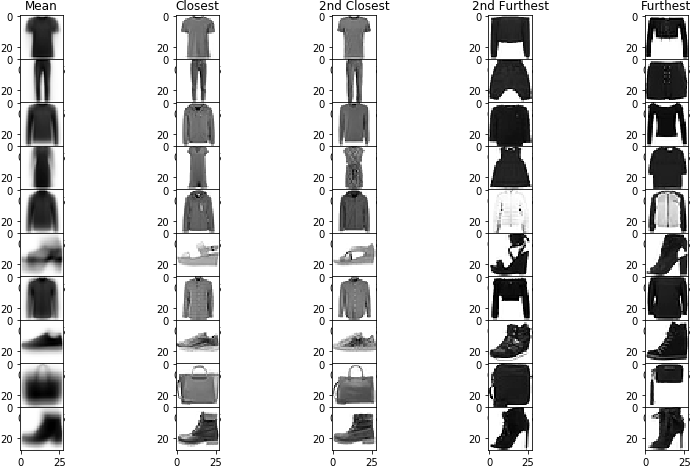
\includegraphics[width=0.75\textwidth]{imgs/1_2.png}
	\end{center}
	The closest samples from each class look very similar to the mean and have light colours. The furthest samples from each class are unusual examples of that class and are dark. This makes sense, as similar images will have usually smaller distances and gray deviations from mean increase the distance less than black ones do. 
  \end{answerbox}



   \end{subquestion}

   % 
   % Q1.3
   \begin{subquestion}{(3 points)
       Apply Principal Component Analysis (PCA) to the data of {\tt
         Xtrn\_nm} using
       \href{https://scikit-learn.org/0.19/modules/generated/sklearn.decomposition.PCA.html}{sklearn.decomposition.PCA},
       and report the variances of projected data for the first five principal
       components in a table. 
       Note that you should use {\tt Xtrn\_nm} instead of {\tt Xtrn}.
           } \label{Q1.pca.variance}



    \begin{answerbox}{15em}
    \begin{center}
    PCA variances of projected data for the first 5 components:
    \begin{tabular}{|c|c|c|c|c|c|}
    \hline 
    K & 1 & 2 & 3 & 4 & 5 \\
    \hline 
    Var & 19.81& 12.11& 4.11& 3.38& 2.62 \\ 
    \hline 
    \end{tabular} 
    \end{center}
    \end{answerbox}
    


   \end{subquestion}

   %==============================
   % Q1.4
   \begin{subquestion}{(3 points)
       Plot a graph of the cumulative explained variance ratio as a
       function of the number of principal components, $K$, where $1
       \le K \le 784$.
       Discuss the result briefly.
     } \label{Q1.plot.pca.variance}
   

      \begin{answerbox}{30em}
        \begin{center}
			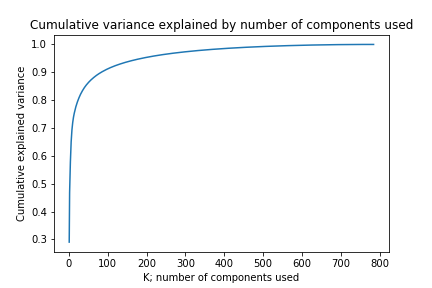
\includegraphics[width=0.75\textwidth]{imgs/1_4.png}
		\end{center}
		\begin{itemize}
		\itemsep -3pt {}
		\item We can see that the cumulative explained variance grows quickly in the $ 1 \leq K  \leq 50 $ interval. Following that, the function increases much more slowly.
		\item Therefore, as $K=50$ PCA components explain $> 86\%$ of the variance, it looks like a good compromise between accuracy and complexity.
		\item It is often useful to plot decision regions on the plane spanned by the first 2 PCA components. They explain only $\sim 53\%$ of the total variance here, so one would need to be cautious when using them.
		\end{itemize}
      \end{answerbox}
  


   \end{subquestion}

   %==============================
   % Q1.5
   \begin{subquestion}{(4 points)
      Display the images of the first 10 principal components in
      a 2-by-5 grid, putting the image of 1st principal component on
      the top left corner, followed by the one of 2nd component to the right.
      Discuss your findings briefly.
     } \label{Q1.disp.pca}
   

      \begin{answerbox}{35em}
         \begin{center}
	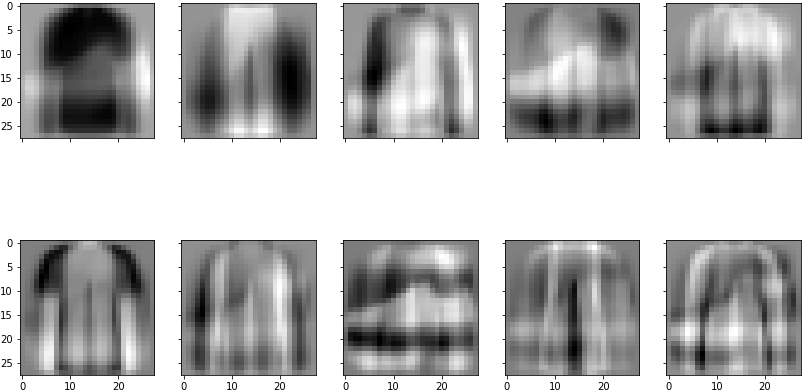
\includegraphics[width=\textwidth]{imgs/1_5.png}
	\end{center}
	
	\begin{itemize}
	\itemsep -3pt {}
	\item We can see that the first component measures how much a picture resembles a shirt, as it has a shape of a t-shirt with gray areas in the shapes of sleeves. This makes sense as there are 4 classes with similar shapes (0: T-Shirt/Top, 2: Pullover, 4: Coat, 6: Shirt). These classes share a shape, so lots of variance can be explained by identifying it. Therefore, it is expected for the most important principal component to identify it (even though PCA is unsupervised).
	\item Out of the other principal components, we can similarly see that the 4-th and the 8-th one identify shoes (and also $5$ and $10$, but to a smaller degree). This makes sense, as there are 3 classes of shoes and they share a unique shape.
	\end{itemize}
      \end{answerbox}
  


   \end{subquestion}

   %==============================
   % Q1.6
   \begin{subquestion}{(5 points)
       Using \texttt{Xtrn\_nm}, 
       for each class and for each number of principal components $K =
       5, 20, 50, 200$, apply dimensionality reduction with PCA to the
       first sample in the class, reconstruct the sample from the
       dimensionality-reduced sample, and 
       report the Root Mean Square Error (RMSE) between the
       original sample in {\tt Xtrn\_nm} and reconstructed one.
     } \label{Q1.6}

     

      \begin{answerbox}{25em}
      \begin{center}
      	RMSE between original and reconstructed samples \\for $K = 5,20,50,200$:\\
      \end{center}
      	\begin{center}
         \begin{tabular}{|c|c|c|c|c|}
         \hline 
        & K=5 & K=20 & K=50 & K=200 \\ \hline
	    Class \#0 & 0.26 & 0.15 & 0.13 & 0.06\\
		Class \#1 & 0.20 & 0.14 & 0.10 & 0.04\\
		Class \#2 & 0.20 & 0.15 & 0.12 & 0.08\\
		Class \#3 & 0.15 & 0.11 & 0.08 & 0.06\\
		Class \#4 & 0.12 & 0.10 & 0.09 & 0.05\\
		Class \#5 & 0.18 & 0.16 & 0.14 & 0.09\\
		Class \#6 & 0.13 & 0.10 & 0.07 & 0.05\\
		Class \#7 & 0.17 & 0.13 & 0.11 & 0.06\\
		Class \#8 & 0.22 & 0.15 & 0.12 & 0.09\\
		Class \#9 & 0.18 & 0.15 & 0.12 & 0.07\\
		\hline
         \end{tabular} 
         \end{center}
      \end{answerbox}
  


   \end{subquestion}
   
   %==============================
   % Q1.7
   \begin{subquestion}{(4 points)
       Display the image for each of the reconstructed samples in
       a 10-by-4 grid, where each row corresponds to a class and
       each row column corresponds to a value of $K=5, \; 20, \; 50, \; 200$.
     } \label{Q1.7}


   

      \begin{answerbox}{52em}
             \begin{center}
	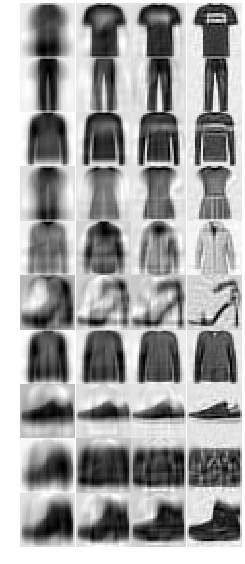
\includegraphics[width=0.5\textwidth]{imgs/1_7.png}
	\end{center}
	We should expect more components to yield better reconstructions and that is visibly the case. The more components we use, the more variance they explain. Therefore, the images should also look more and more realistic (less blurred) and they do.
      \end{answerbox}
  


   \end{subquestion}
   %==============================
   %
   %==============================
   % Q1.8
   \begin{subquestion}{(4 points)
       Plot all the training samples (\texttt{Xtrn\_nm}) on the
       two-dimensional PCA plane you obtained in \refQ{Q1.pca.variance}, where each sample is
       represented as a small point with a colour specific to the class of
       the sample.  Use the 'coolwarm' colormap for plotting.
     } \label{Q1.8}


   

      \begin{answerbox}{40em}
         \begin{center}
	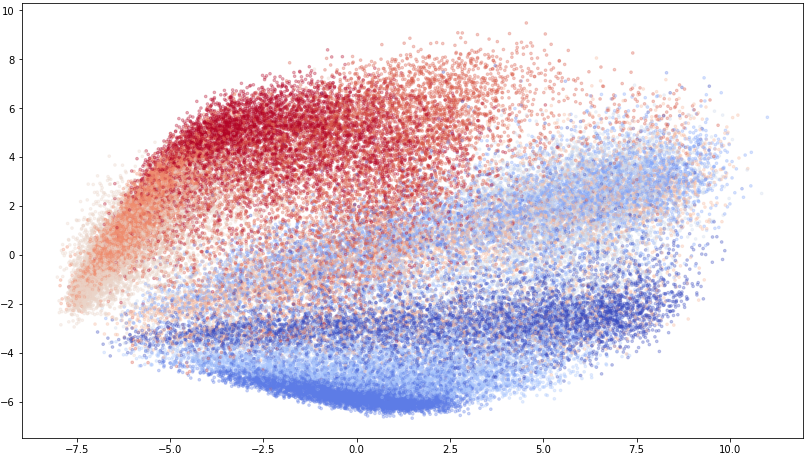
\includegraphics[width=\textwidth]{imgs/1_8.png}
	\end{center}
	\begin{itemize}
	\itemsep -3pt {}
	\item The classes are not fully separated as we can, for example, see that red and blue samples mix in the middle.
	\item We can also obersve that the bottom is dominated by blue samples and the top by red/orange ones. 
	\item This suggests that the first PCA component has little discriminatory power (but explains more of the variance), while the second PCA component actually distinguishes between classes (given the first component).
	\end{itemize}
      \end{answerbox}
  


   \end{subquestion}
   %
   %==============================
   

\end{question}
%%%%%%%%%%%%%%%%%%%%%%%%%%%%%%%%%%%%%%%%%%%%%%%%%%%%%%%%%%%%%%%%%%%%%%%%%%%%%%
%============================================================================%
%%%%%%%%%%%%%%%%%%%%%%%%%%%%%%%%%%%%%%%%%%%%%%%%%%%%%%%%%%%%%%%%%%%%%%%%%%%%%%
\clearpage
%
% Question 2
%
\begin{question}{(25 total points) Logistic regression and SVM}

  \questiontext{In this question we will explore 
    classification of image data with logistic regression and support
    vector machines (SVM) and visualisation 
    of decision regions.
  }
  


  \medskip
   %==============================
   % Q2.1
   \begin{subquestion}{(3 points)
       Carry out a classification experiment with
       \href{https://scikit-learn.org/0.19/modules/generated/sklearn.linear\_model.LogisticRegression.html}{multinomial logistic regression},
       and report the classification accuracy and confusion matrix (in
       numbers rather than in graphical representation such as heatmap)
       for the test set.
     } \label{Q2.1}


   

      \begin{answerbox}{30em}
      Accuracy: 84.01\% \\
    		\begin{tabular}{|c|c|c|c|c|c|c|c|c|c|c|c|}
      		\hline 
      		\multicolumn{11}{|c|}{Confusion Matrix}\\
      		\multicolumn{11}{|c|}{$(C_{ij} = $ samples known to be in class $i$ and predicted to be in $j$)}
      		 \\ \hline
\ \ \ \ \ \ \ \ & 0 & 1 & 2 & 3 & 4 & 5 & 6 & 7 & 8 & 9\\ \hline
0 & 819 & 3 & 15 & 50 & 7 & 4 & 89 & 1 & 12 & 0 \\ \hline 
1 & 5 & 953 & 4 & 27 & 5 & 0 & 3 & 1 & 2 & 0 \\ \hline 
2 & 27 & 4 & 731 & 11 & 133 & 0 & 82 & 2 & 9 & 1 \\ \hline 
3 & 31 & 15 & 14 & 866 & 33 & 0 & 37 & 0 & 4 & 0 \\ \hline 
4 & 0 & 3 & 115 & 38 & 760 & 2 & 72 & 0 & 10 & 0 \\ \hline 
5 & 2 & 0 & 0 & 1 & 0 & 911 & 0 & 56 & 10 & 20 \\ \hline 
6 & 147 & 3 & 128 & 46 & 108 & 0 & 539 & 0 & 28 & 1 \\ \hline 
7 & 0 & 0 & 0 & 0 & 0 & 32 & 0 & 936 & 1 & 31 \\ \hline 
8 & 7 & 1 & 6 & 11 & 3 & 7 & 15 & 5 & 945 & 0 \\ \hline 
9 & 0 & 0 & 0 & 1 & 0 & 15 & 1 & 42 & 0 & 941
			\\\hline
      		\end{tabular} 
      \end{answerbox}
  


   \end{subquestion}
   %
   % ==============================
   %
   %==============================
   % Q2.2
   \begin{subquestion}{(3 points)
       Carry out a classification experiment with
       \href{https://scikit-learn.org/0.19/modules/generated/sklearn.svm.SVC.html}{SVM classifiers}, and report the
       mean accuracy and confusion matrix (in numbers) for the test
       set.
     } \label{Q2.2}


   

      \begin{answerbox}{30em}
             Accuracy: 84.61\% \\
    		\begin{tabular}{|c|c|c|c|c|c|c|c|c|c|c|c|}
      		\hline 
      		\multicolumn{11}{|c|}{Confusion Matrix}\\
      		\multicolumn{11}{|c|}{$(C_{ij} = $ samples known to be in class $i$ and predicted to be in $j$)}
      		 \\ \hline
\ \ \ \ \ \ \ \ & 0 & 1 & 2 & 3 & 4 & 5 & 6 & 7 & 8 & 9\\ \hline
0 & 845 & 2 & 8 & 51 & 4 & 4 & 72 & 0 & 14 & 0 \\ \hline 
1 & 4 & 951 & 7 & 31 & 5 & 0 & 1 & 0 & 1 & 0 \\ \hline 
2 & 15 & 2 & 748 & 11 & 137 & 0 & 79 & 0 & 8 & 0 \\ \hline 
3 & 32 & 6 & 12 & 881 & 26 & 0 & 40 & 0 & 3 & 0 \\ \hline 
4 & 1 & 0 & 98 & 36 & 775 & 0 & 86 & 0 & 4 & 0 \\ \hline 
5 & 0 & 0 & 0 & 1 & 0 & 914 & 0 & 57 & 2 & 26 \\ \hline 
6 & 185 & 1 & 122 & 39 & 95 & 0 & 533 & 0 & 25 & 0 \\ \hline 
7 & 0 & 0 & 0 & 0 & 0 & 34 & 0 & 925 & 0 & 41 \\ \hline 
8 & 3 & 1 & 8 & 5 & 2 & 4 & 13 & 4 & 959 & 1 \\ \hline 
9 & 0 & 0 & 0 & 0 & 0 & 22 & 0 & 47 & 1 & 930
			\\\hline
      		\end{tabular} 
      \end{answerbox}
  


   \end{subquestion}
   %
   % ==============================
   %
   %==============================
   % Q2.3
   \begin{subquestion}{(6 points)
       We now want to visualise the decision regions for the logistic
       regression classifier we trained in \refQ{Q2.1}.
     } \label{Q2.3}


   

      \begin{answerbox}{35em}
                  \begin{center}
	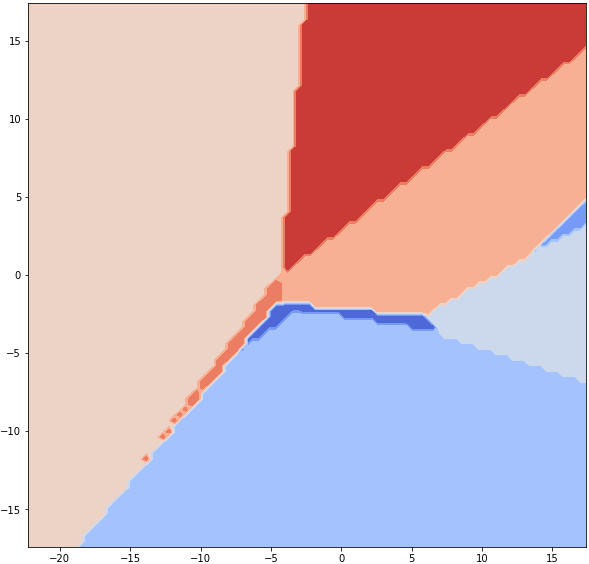
\includegraphics[width=0.65\textwidth]{imgs/2_3.png}
	\end{center}
	\begin{itemize}
	\itemsep -3pt {}
	\item Each class has a linear boundary here. This makes sense, as logistic regression is a linear classifier and PCA coordinates are linear combinations of original coordinates. Irregularities are probably caused by the numerical approximation.\
\item As expected (first two components explain most of the variance), the main differences are visibly captured.
%	\item Class 9 does not appear here. This means that no reconstructions of points from the PCA plane are classified as class 9. More intutively, first two components don't capture the uniqueness of class 9.
	\end{itemize}
      \end{answerbox}
  


   \end{subquestion}
   %
   % ==============================
   %
   %==============================
   % Q2.4
   \begin{subquestion}{(4 points)
       Using the same method as the one above, plot the decision regions for
       the SVM classifier you trained in \refQ{Q2.2}.
       Comparing the result with that you obtained in \refQ{Q2.3}, discuss your
       findings briefly.
     } \label{Q2.4}
   

      \begin{answerbox}{35em}
                           \begin{center}
	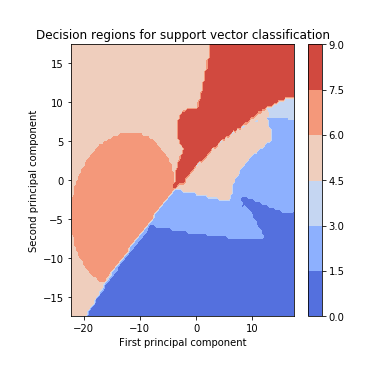
\includegraphics[width=0.65\textwidth]{imgs/2_4.png}
	\end{center}
	\begin{itemize}
	\itemsep -3pt {}
	\item Unlike for logistic regression, decision boundaries here are non-linear. This makes sense as SVMs are not linear classifiers (not for RBF kernels).
	\item There are significant differences in decision regions between the SVM model and logistic regression.
	\item As expected (first two components explain most of the variance), the main differences are visibly captured here as well.
	%\item Class 9 does not appear here. This means that no reconstructions of points from the PCA plane are classified as class 9. More intutively, first two components don't capture the uniqueness of class 9.
	\end{itemize}
      \end{answerbox}
  


   \end{subquestion}
   %
   % ==============================
   %

   %==============================
   % Q2.5
   \begin{subquestion}{(6 points)
       We used default parameters for the SVM in \refQ{Q2.2}.
       We now want to tune the parameters by using cross-validation.
       To reduce the time for experiments, you pick up the first 1000
       training samples from each class to create \texttt{Xsmall}, so that \texttt{Xsmall}
       contains 10,000 samples in total. Accordingly, you create
       labels, \texttt{Ysmall}.
     } \label{Q2.5}


   

      \begin{answerbox}{30em}
           \begin{center}
	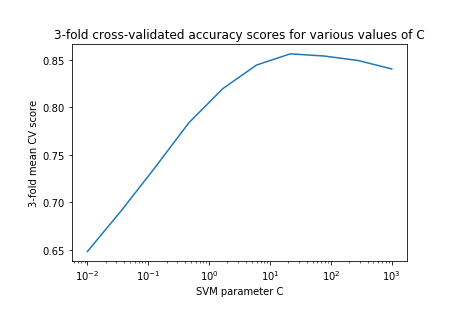
\includegraphics[width=0.85\textwidth]{imgs/2_5.png}
	\end{center}
	The highest mean 3-fold CV accuracy score was $\sim 85.65\%$. \\
	It was realised by $C=10^{4/3} \approx 21.54$.
      \end{answerbox}
  


   \end{subquestion}
   %
   % ==============================
   %
   %==============================
   % Q2.6
   \begin{subquestion}{(3 points)
       Train the SVM classifier on the whole training set by using the
       optimal value of $C$ you found in \refQ{Q2.5}. 
     } \label{Q2.6}


       

      \begin{answerbox}{10em}
         Classification accuracy for $C=10^{4/3}$ is approximately:
         \begin{itemize}
        	\itemsep -3pt {}
        	\item 90.84\% for the training data
        	\item 87.65\% for the test data
         
		\end{itemize}          
      \end{answerbox}
  


   \end{subquestion}
   %
   % ==============================
   %
%
%

\end{question}
%%%%%%%%%%%%%%%%%%%%%%%%%%%%%%%%%%%%%%%%%%%%%%%%%%%%%%%%%%%%%%%%%%%%%%%%%%%%%%
%============================================================================%
%%%%%%%%%%%%%%%%%%%%%%%%%%%%%%%%%%%%%%%%%%%%%%%%%%%%%%%%%%%%%%%%%%%%%%%%%%%%%%
\clearpage
%
% Question 3
%

\begin{question}{(20 total points) Clustering and Gaussian Mixture Models}  


  \questiontext{In this question we will explore K-means clustering,
    hierarchical clustering, and GMMs.
  }
  


  \medskip
   %==============================
   % Q3.1
   \begin{subquestion}{(3 points)
       Apply k-means clustering on {\tt Xtrn} for $k = 22$, where we use
       \href{https://scikit-learn.org/0.19/modules/generated/sklearn.cluster.KMeans.html}{sklearn.cluster.KMeans}
       with the parameters {\tt n\_clusters=22} and {\tt random\_state=1}.
       Report the sum of squared distances of samples to their closest
       cluster centre, and the number of samples for each cluster.
     } \label{Q3.1}
   

      \begin{answerbox}{35em}
         Sum of squared distances to their closest cluster centre (inertia): $38185.82$.
\begin{center}
\begin{tabular}{|c|c|}
\hline 
Cluster & Cluster \\
number & size \\\hline
0 & 1018 \\\hline
1 & 1125 \\\hline
2 & 1191 \\\hline
3 & 890 \\\hline
4 & 1162 \\\hline
5 & 1332 \\\hline
6 & 839 \\\hline
7 & 623 \\\hline
8 & 1400 \\\hline
9 & 838 \\\hline
10 & 659 \\\hline
11 & 1276 \\\hline
12 & 121 \\\hline
13 & 152 \\\hline
14 & 950 \\\hline
15 & 1971 \\\hline
16 & 1251 \\\hline
17 & 845 \\\hline
18 & 896 \\\hline
19 & 930 \\\hline
20 & 1065 \\\hline
21 & 1466 \\\hline

\hline 
\end{tabular} \end{center}
      \end{answerbox}
  


   \end{subquestion}
   %
   % ==============================
   %
   %==============================
   % Q3.2
   \begin{subquestion}{(3 points)
       Using the training set only,
       calculate the mean vector for each language, and plot the mean
       vectors of all the 22 languages on a 2D-PCA plane, where you
       apply PCA on the set of 22 mean vectors without applying
       standardisation.  
       On the same figure, plot the cluster centres obtained in \refQ{Q3.1}.
     } \label{Q3.2}

   

      \begin{answerbox}{35em}
                    \begin{center}
	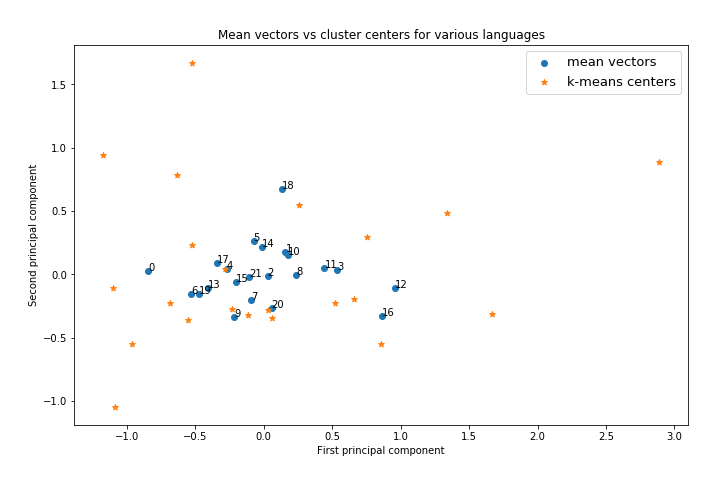
\includegraphics[width=\textwidth]{imgs/3_2.png}
	\end{center}
	\begin{itemize}
	\itemsep -3pt {}
	\item The mean vectors and clusters are similar. But, clusters are more spread out. This was to be expected as outliers from different languages will be grouped together in k-means, while they will cancel each other in means.
	\item If the distributions of points for each language were in close neighbourhoods of  mean vectors, we would expect the k-means centers to be very close to mean vectors. This is not the case here, so these distributions must often overlap.
	\end{itemize}
      \end{answerbox}
  


   \end{subquestion}
   %
   % ==============================
   %
   %==============================
   % Q3.3
   \begin{subquestion}{(3 points)
       We now apply hierarchical clustering on the training data set
       to see if there are any structures in the spoken languages.
     } \label{Q3.3}


     

      \begin{answerbox}{35em}
           \begin{center}
	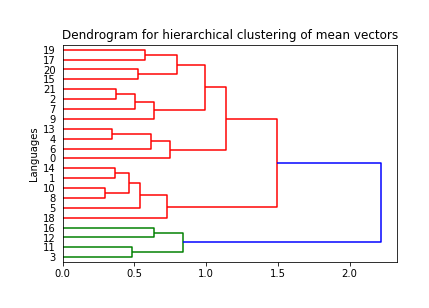
\includegraphics[width=\textwidth]{imgs/3_3.png}
	\end{center}
	\begin{itemize}
	\itemsep -3pt {}
	\item We can see that there are 4 languages that are diametrically different from the rest ($\{3,11,12,16\}$), as they are only merged with the rest in the final cluster and the distance along the final U-link is very long (represents distance here).
	\item More generally, we can see that the lengths of U-links do not vary too much. For example, there are no pairs of unusually similar languages. 
	\end{itemize}
      \end{answerbox}
  


   \end{subquestion}
   %
   % ==============================
   %
   %==============================
   % Q3.4
   \begin{subquestion}{(5 points)
       We here extend the hierarchical clustering done in \refQ{Q3.3} by
       using multiple samples from each language.
     } \label{Q3.4}


   

      \begin{answerbox}{50em}
                  \begin{center}
	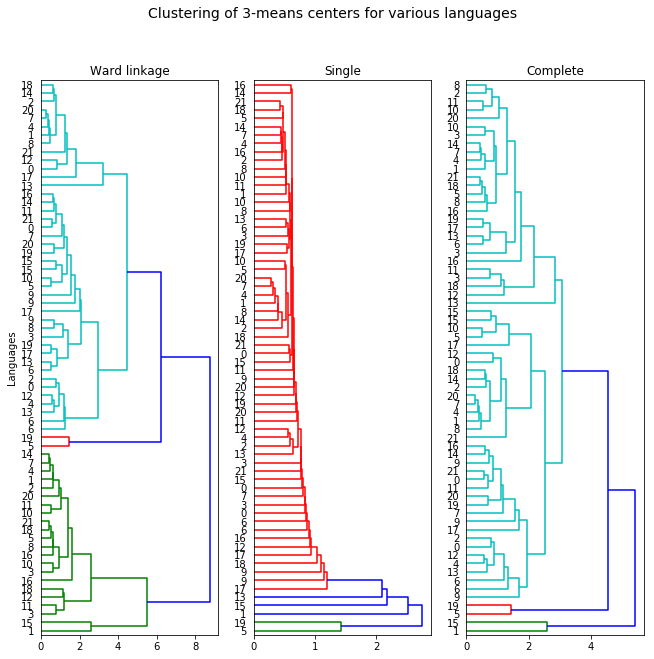
\includegraphics[width=0.99\textwidth]{imgs/3_4.png}
	\end{center}
	\begin{itemize}
	\itemsep -3pt {}
	\item We can see that different linkage methods produce considerably different dendrograms. They are also all unbalanced.
	\item Ward linkage produced a green cluster which approximately contains one cluster centre per language. This suggests that this cluster shares a language-universal attribute. For example, it might be the set of cluster centers of recordings of mostly children.
	\item Unlike Ward, single and complete linkages produced single clusters that cover nearly all of the language cluster centers. This shows that there a small minority of cluster centers which are outliers (all among \{1,5,13,15,19\}).
	\end{itemize}
      \end{answerbox}
  


   \end{subquestion}
   %
   % ==============================
   %
   %==============================
   % Q3.5
   \begin{subquestion}{(6 points)
       We now consider Gaussian mixture model (GMM), whose
       probability distribution function (pdf) is given as
       a linear combination of Gaussian or normal distributions, i.e.,
     } \label{Q3.5}




      \begin{answerbox}{30em}
            \begin{center}
			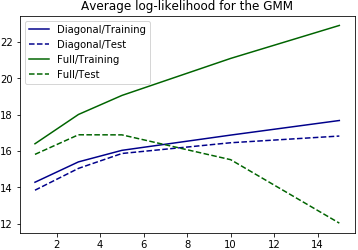
\includegraphics[width=0.68\textwidth]{imgs/3_5.png}
			\begin{tabular}{|c|c|c|c|c|c|}

			\hline 
 & 1 & 3 & 5 & 10 & 15\\ \hline
Diagonal/Training & 14.28 & 15.40 & 16.01 & 16.88 & 17.68 \\ \hline
Diagonal/Test & 13.84 & 15.04 & 15.91 & 16.73 & 17.03 \\ \hline
Full/Training & 16.39 & 18.05 & 19.19 & 21.02 & 22.99 \\ \hline
Full/Test & 15.81 & 17.00 & 16.64 & 14.72 & 11.78 \\ \hline

			\end{tabular} 
		\end{center}
	As expected, the most general model (full covariance matrix) fits the training data best. Also, this model begins to overtrain for $K>3$. The less general model (diagonal covariance matrix) has a weaker fit, but doesn't overtrain for bigger $K$s.

      \end{answerbox}
  


   \end{subquestion}
   %
   %==============================

   % ==============================
   
\end{question}
\end{document}
